\chapter{ORCA: A Unified Framework for Declarative Observability}

\section{Motivation: Programmable and Real-time Cluster Observability}

% Ideal observability enables querying cluster state to materialize complex views on demand. CARP
% demonstrates this capability for data path optimization, using state reconstruction to inform
% online range partitioning. Our AMR work reveals the urgent need for such capability on the compute
% path, where performance tuning requires seeing past system noise to identify root causes. Both
% point toward a unified solution: a general-purpose framework for materializing views of
% distributed system state from streaming data.

Both CARP and our work on AMR placement reveal a persistent and recurring need to reconstruct
cluster state to synthesize views that enable better decision-making.
CARP automatically uses this reconstructed state to inform online range partitioning, and our AMR
work reveals the urgent need for such capability on the compute path, where disambiguating between
load imbalance, system variability,a nd execution startrategies is essential for computational
efficiency.
While we evolved a telemetry workflow in our AMR work, it was still ad-hoc and limited.
From these experiences, we derive three requirements for powerful observability capabilities
deployable in production clusters.


\begin{itemize}
  \item \textbf{Real-time and Coordinated Analytics}
        Framework must be able to produce insights in realtime with minimal application overhead, as well
        as optionally persist detailed telemetry for offline analysis.
        This requires coordinated collection of timestep-wise telemetry from all ranks.

  \item \textbf{Complete Programmability.}
        Observability workflows require collecting and aggregating data from different data sources, with
        different schemas, and different aggregation strategies in different contexts.
        Imposing arbitrary constraints on any of these limits the applicability of the framework.


  \item \textbf{Interactivity}
        It is necessary to be able to change aggregations and data sources mid-execution.
        In the common case, summary statistics are sufficient to monitor for the presence of problems.
        In the presence of problems, it is necessary to be able to enable more telemetry to localize the
        root cause of the problem.
        Such a capability would enable a full spectrum of workflows upto tracing.
        Instead of imposing fixed costs for data collection as with tracing, this allows for the costs to
        be proportional to workflow requirements.
\end{itemize}

\section{Background: The Observability Gap in BSP Systems}

Currently, comprehensive tracing is the only method that preserves the fine-grained, coordinated
event data needed to diagnose complex performance issues in large-scale BSP systems.
However, the high application overhead, unstructured and analytics-unfriendly output, and delayed
feedback from post-processing make tracing impractical for production use.
As clusters and their resource footprints continue to grow, these limitations become more acute,
necessitating a ground-up rethinking of observability architectures to keep pace with modern system
demands.

Profiling and sampling tools, while lower overhead, impose arbitrary fixed collection and
aggregation patterns that obscure the structure of underlying problems and mask important temporal
or spatial correlations.
Time Series Databases (TSDBs), widely used for metrics in distributed services, are not a direct
fit for scalable BSP observability, as they cannot support low-overhead coordinated collection,
dynamic workflows, or aggressive in-situ filtering.
These issues mean that gaps in cluster efficiency persist not due to unsolved algorithmic
bottlenecks, but because of persistent limitations in what can be observed, analyzed, and acted on
in real time.



\section{ORCA Architecture}

ORCA is designed to address the challenges of scalable, real-time observability in large parallel
systems via programmable aggregation and control paths.
The framework enables users to express analytic intent as SQL over telemetry.
Unlike tracing, which collects and stores all event data, ORCA leverages distributed query planning
to transfer only the data necessary to materialize each requested view.
Its control semantics enable dynamic transitions between different views at runtime, supporting
interactive, low-overhead workflows.
Below, we briefly describe the core components of the ORCA architecture.

\begin{itemize}
  \item \textbf{Tree-Based Overlay Network (TBON):}
        ORCA organizes application ranks into a logical tree-based overlay with a controller at the root, a
        tier of aggregators, optionally a tier of lead ranks (aggregating within node groups), and
        application ranks as leaves.
        Aggregators handle data collection from a subset of ranks, using RDMA for data transfer when
        available.

  \item \textbf{Distributed Query Planning:}
        Telemetry is represented in Apache Arrow columnar format, and the overlay implements distributed
        query planning using Apache Datafusion.
        Projection, filtering, and partial aggregation are pushed down to lower tiers, so only necessary
        data is transferred up the tree.

  \item \textbf{Timestep-Linked Two-Phase Commit (TS2PC) Control Path:}
        ORCA implements a control path using the TS2PC protocol.
        TS2PC is an asynchronous protocol that enables control actions to be applied consistently at a
        specified timestep across all ranks.
        This provides low-overhead replicated state machine semantics and supports dynamic observability
        workflows.
\end{itemize}

\section{Potential Usecases and Impact}

ORCA enables a range of use cases across high-performance computing and machine learning workflows,
while providing a foundation for broader analytics and control in the future.

\paragraph{HPC Workloads}
ORCA enables continuous, always-on observability for large-scale simulation codes.
Unlike traditional workflows that require choosing between lightweight profiling and expensive
tracing, ORCA supports a seamless spectrum: developers can inject detail dynamically and escalate
from low-overhead monitoring to deep, on-demand root-cause analysis as needed.
This removes silos between telemetry collection modes and provides actionable insight without
workflow disruption.

\paragraph{ML Workloads}
Distributed ML workloads, because of their shared BSP characteristics, present similar performance
and observability challenges as HPC codes~\cite{Gangi2024:RDMA}.
For example, PyTorch~\cite{Paszk2019:PyTorch} enables tracing each node using Kineto, but no mechanism exists to aggregate
per-node telemetry into global views.
Delayed feedback, lack of analytical capabilities, and the other limitations studied for HPC apply
equally here.
Beyond performance, recent ML research has emphasized the need for runtime observability over
application state to enforce correctness invariants~\cite{Jiang2025:TrainingwithConfidence}.
We find that ORCA naturally accommodates such use cases because of its focus on programmability,
enabling a common substrate for multiple forms of observability.

\paragraph{Longer-Term Vision}
ORCA's software-based architecture --- incorporating open standards such as Apache
Arrow~\cite{:ApacheArrow}, Datafusion~\cite{Lamb2024:DataFusion}, and
Mercury~\cite{Souma2013:MercuryRPC} over libfabric --- makes it naturally extensible.
Many scientific analyses depend on multidimensional and sometimes unstructured meshes, which are
not straightforward to represent in the relational model of standard SQL.
Prior work~\cite{:TileDB,Lee2004:MeshSQL,Kerst2011:SciQL,Rezae2014:UnstructuredMeshAlgebra} provides clear paths for extending SQL to cover these data types, and ORCA is is
amenable to absorbing these capabilities, enabling in-situ visualization workflows within the same
pipeline.
Previous work has
also shown how accelerators can be used for in-situ analysis on Arrow
data~\cite{Liu2022:ProcessingParticleData, Ulmer2023:ExtendingComposableData}, and ORCA makes this
practical by exposing accelerators and smart network resources as nodes within its dataflow graph.
This enables a unified analytics and control fabric for scientific and data-intensive computing
ecosystems to emerge organically over time.

\begin{figure}[h]
  \centering
  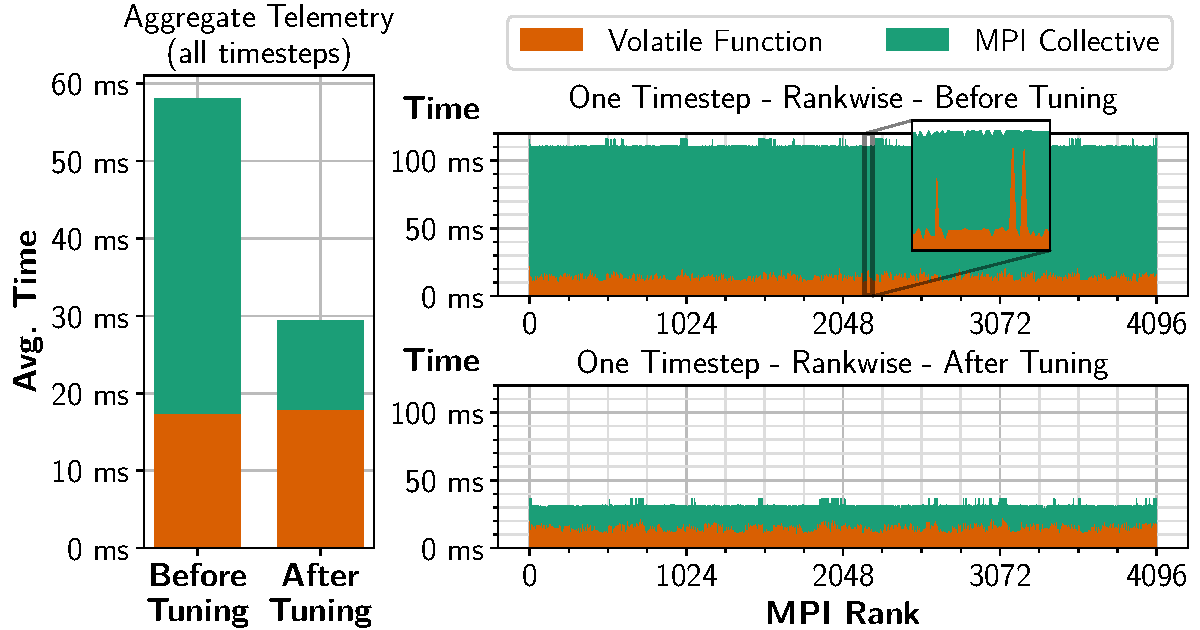
\includegraphics[width=0.7\textwidth,trim=0cm 0cm 0cm 0cm,clip
  ]{data/figs/amr_lesson_volfunc_v2_short_zoom.pdf}
  \caption{AMR lesson.}
  \label{fig:orca-spike}
\end{figure}

\begin{figure}[h]
  \centering
  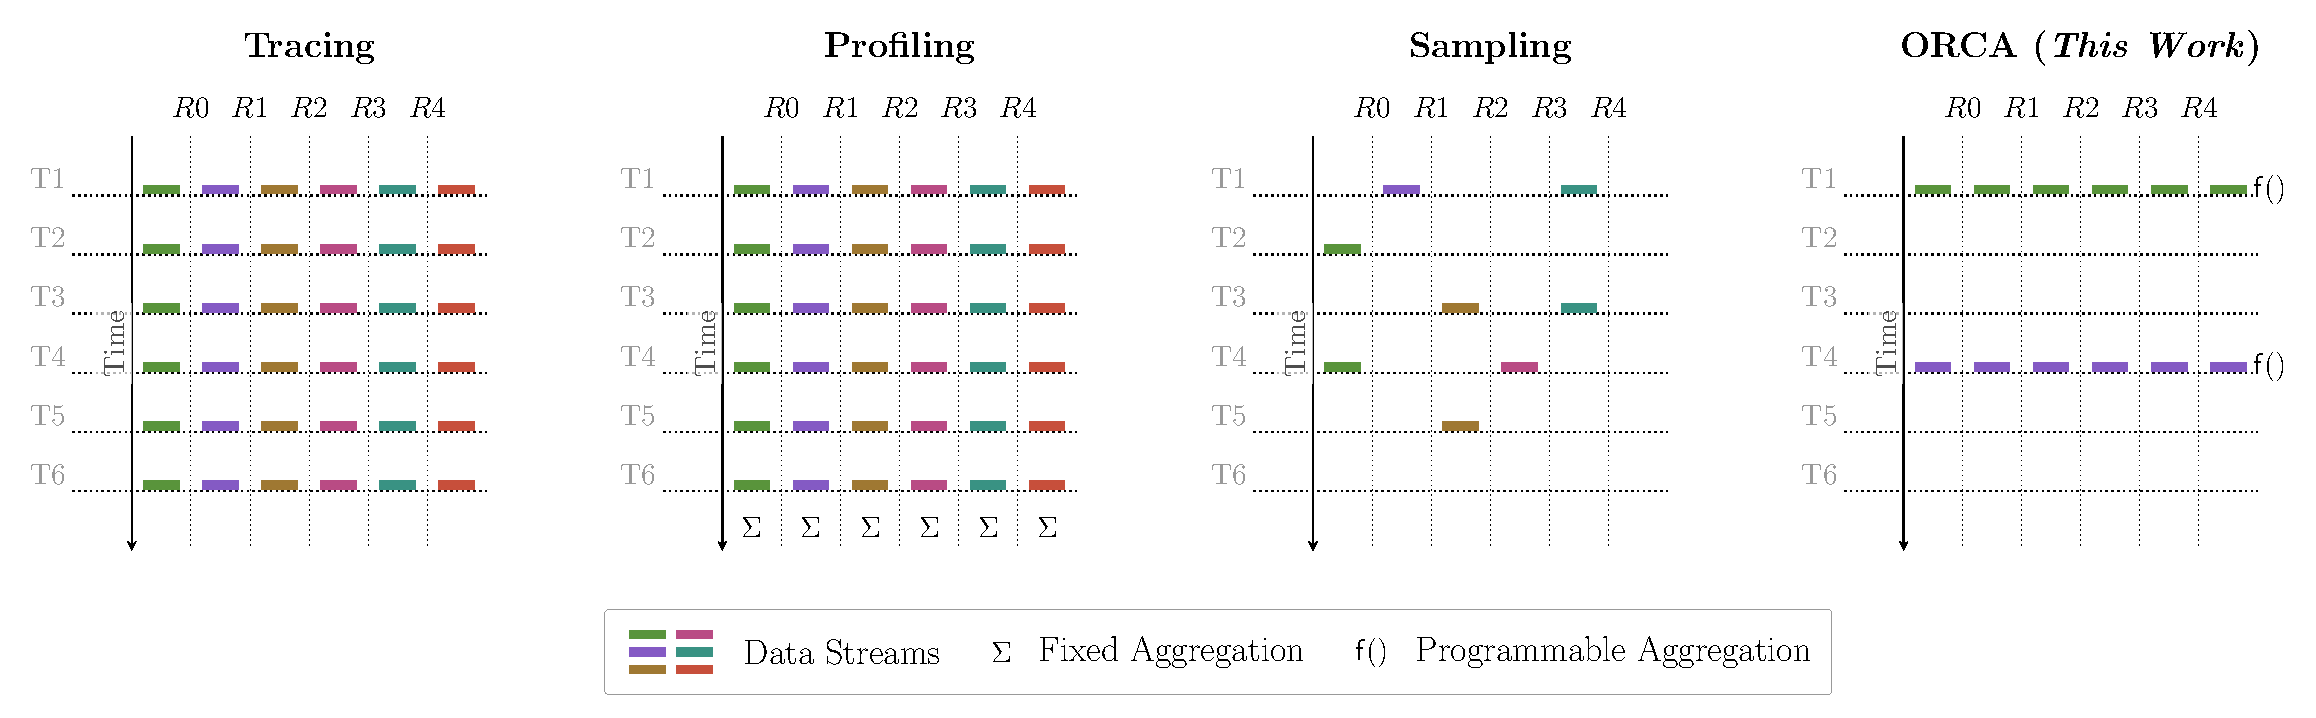
\includegraphics[width=\textwidth,trim=0cm 0cm 0cm 0cm,clip
  ]{data/figs/orca_sampling.pdf}
  \caption{Sampling.}
  \label{fig:orca-approaches}
\end{figure}

\begin{figure}[h]
  \centering
  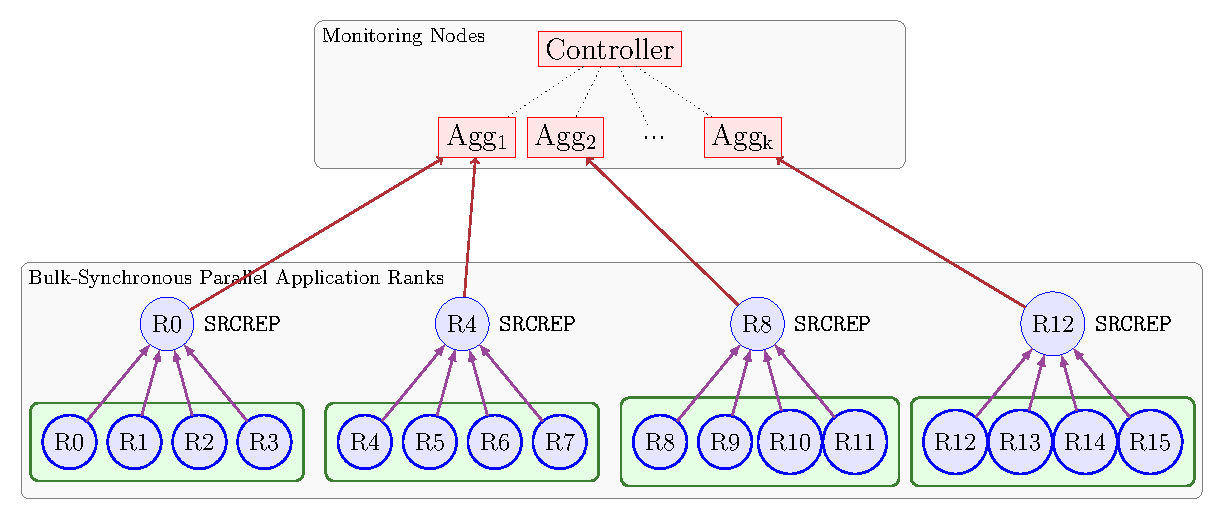
\includegraphics[width=0.7\textwidth,trim=0cm 0cm 0cm 0cm,clip
  ]{data/figs/orca_overlay-agg-new.pdf}
  \caption{ORCA architecture.}
  \label{fig:orca-overlay}
\end{figure}